\begin{figure} %[htbp]
  \begin{subfigure}{.32\textwidth}
   \centering
   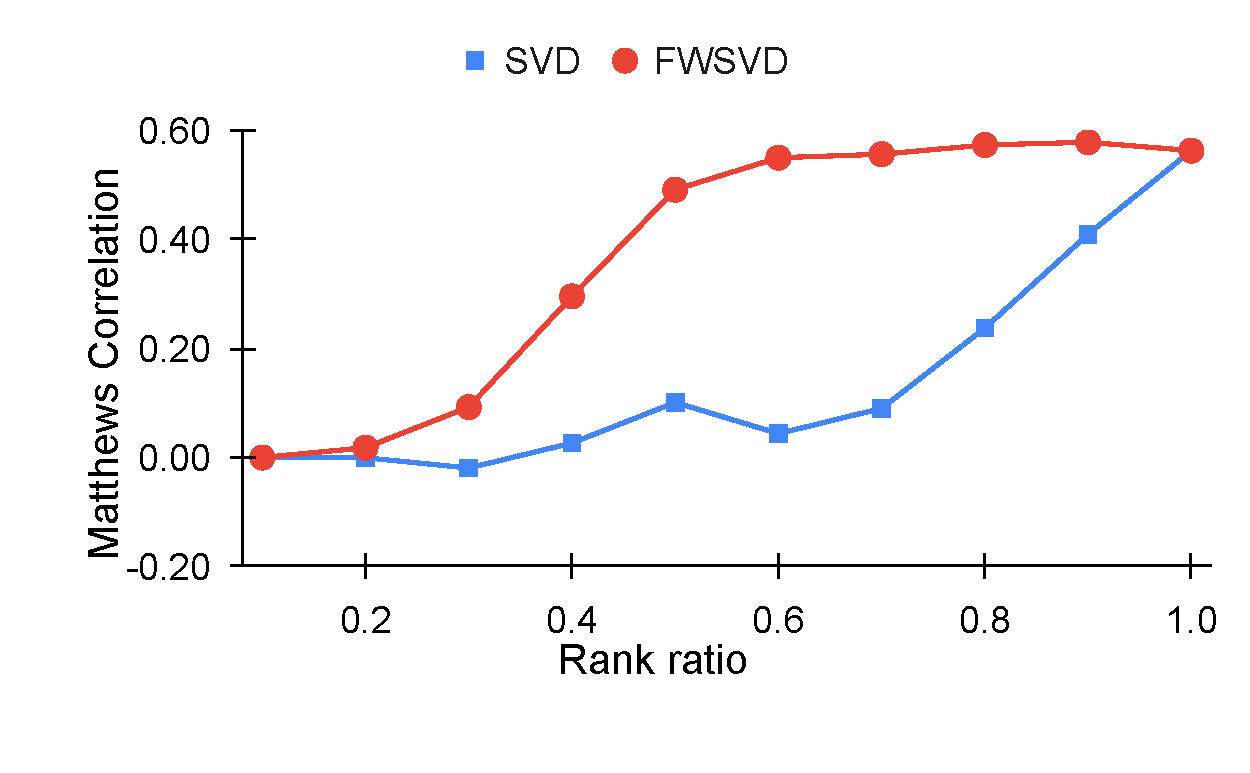
\includegraphics[clip, trim=0cm 0.5cm 0cm 0.5cm,width=\textwidth]{figures/exp_fig1_COLA.pdf}
       \caption{COLA}
       \label{fig:rank:cola}
       \end{subfigure}
\begin{subfigure}{.32\textwidth}
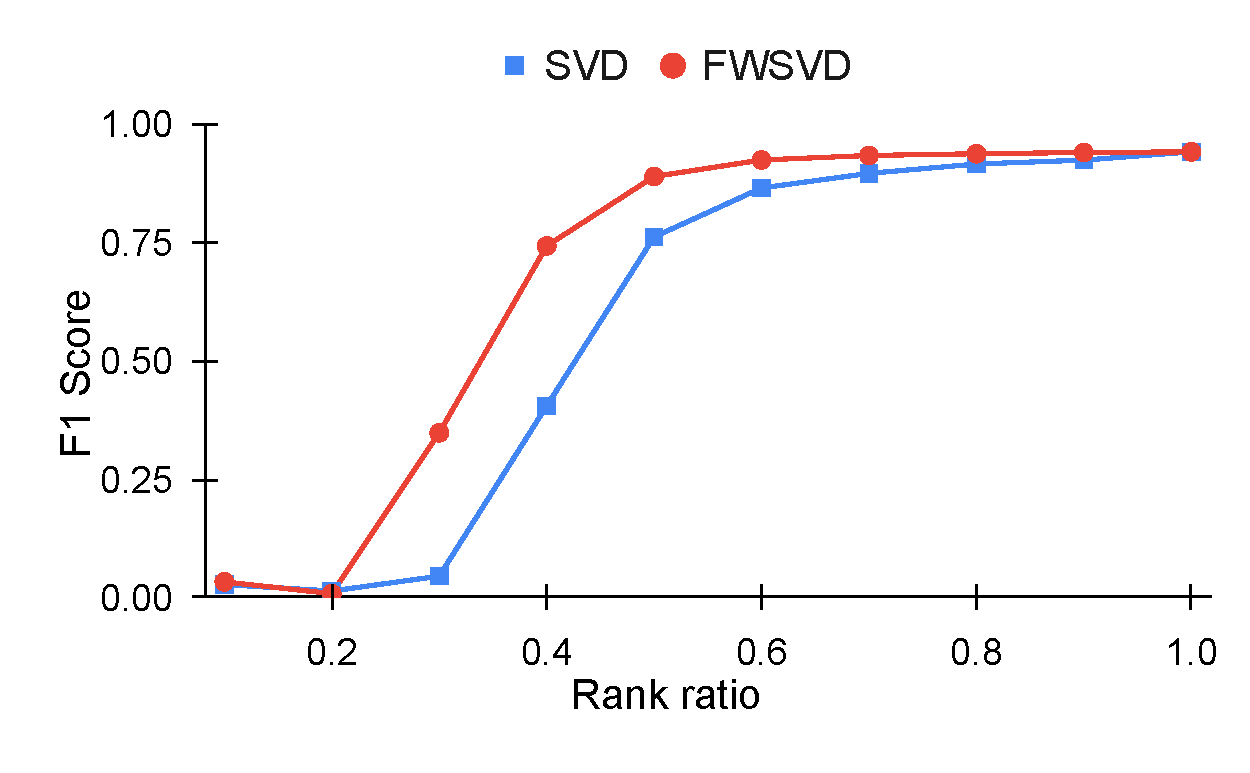
\includegraphics[clip, trim=0cm 0.5cm 0cm 0.5cm,width=\textwidth]{figures/exp_fig1_NER.pdf}
\centering
  \caption{NER (CoNLL-2003)}
   \label{fig:rank:ner}
\end{subfigure}
\begin{subfigure}{.32\textwidth}
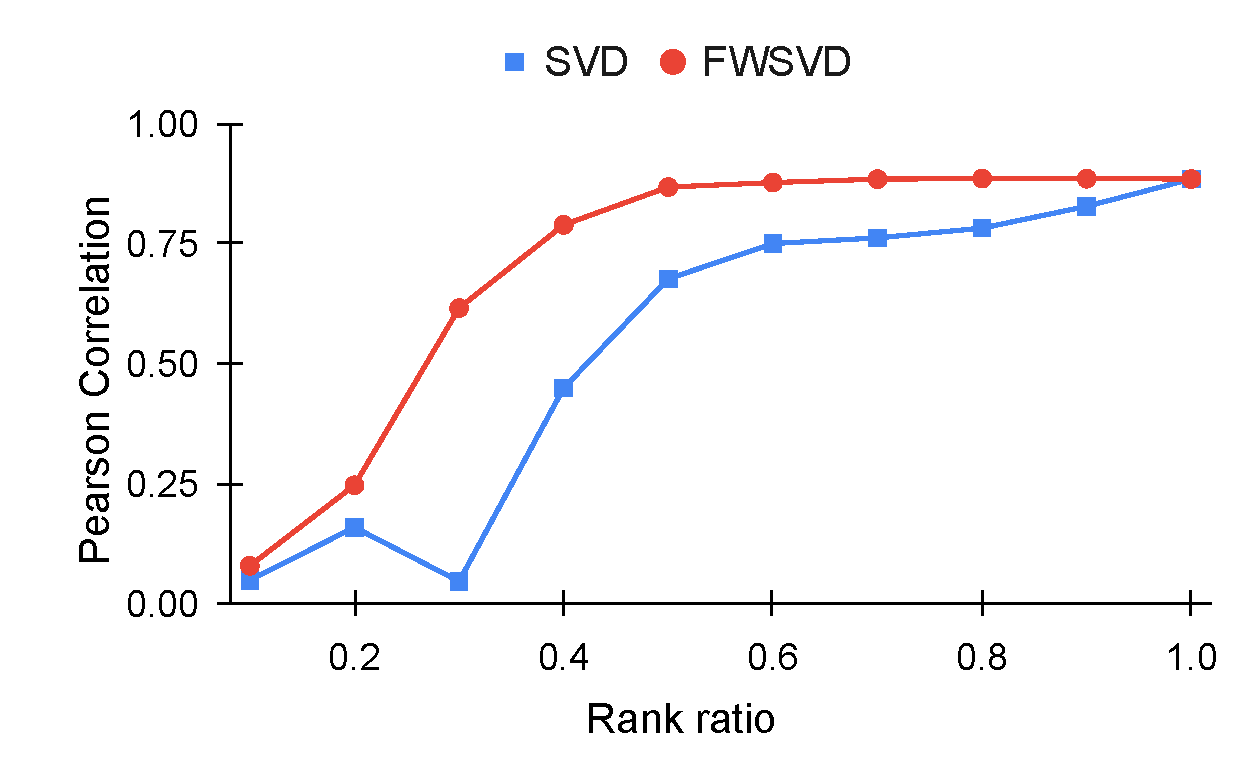
\includegraphics[clip, trim=0cm 0.5cm 0cm 0.5cm,width=\textwidth]{figures/exp_fig1_STSB.pdf}
\centering
  \caption{STS-B}
   \label{fig:rank:stsb}
\end{subfigure}
\caption{FWSVD versus SVD by varying the ratio of reserved ranks. The model with a rank ratio 1.0 indicates the full-rank reconstruction with the same accuracy as the original model (\ie, the $L^t$ in Figure \ref{fig:scheme}). Note that all the models here do not have fine-tuning after factorization. 
% \vspace{-0.3cm}
}
\label{fig:rank}
\end{figure}